\documentclass[11pt]{article}
\usepackage[utf8]{inputenc}
\usepackage[T1]{fontenc}
\usepackage{multirow}
\usepackage{amsmath}
\usepackage{amsfonts}
\usepackage{amssymb}
\usepackage[version=4]{mhchem}
\usepackage{stmaryrd}
\usepackage{graphicx}
\usepackage[export]{adjustbox}
\graphicspath{ {./images/} }

\begin{document}
\section*{Reading}
Problems with Internal Rate of Return

This section begins with two major types of complications in the computation and interpretation of IRRs. In the previous section, IRR was easily computed and interpreted because of the simplified cash flow patterns used and because the investment was being viewed in isolation. The first complication arises when an investment offers a complex cash flow pattern other than the traditional pattern of a cash outflow to initiate an investment, followed only by cash inflows until the investment is terminated. The second complication occurs when investments must be compared to see which is preferred. These two complications are addressed in the first half of this section, followed by a brief discussion of other challenges.

\section*{Complex Cash Flow Patterns}
For the purposes of this analysis of IRRs, a complex cash flow pattern is an investment involving either borrowing or multiple sign changes. A borrowing type cash flow pattern begins with one or more cash inflows and is followed only by cash outflows. An example of the borrowing pattern is when an investment such as a real estate project is sold and leased back. The divestment generates current cash at the cost of future cash outflows and may be viewed as a form of borrowing. A multiple sign change cash flow pattern is an investment where the cash flows switch over time from inflows to outflows, or from outflows to inflows, more than once. An example of a multiple sign change investment would be a natural resource investment involving (1) negative initial cash flows from purchasing equipment and land to set up an operation such as mining, (2) positive interim cash flows from operations, and (3) negative terminal cash flows from ceasing operation and restoration expenses. The next exhibit illustrates the complex cash flow patterns.

\begin{center}
\begin{tabular}{|c|c|c|c|c|c|c|}
\hline
\multirow[b]{2}{*}{Cash Flow Pattern} & \multicolumn{6}{|c|}{Time Period} \\
\hline
 & 0 & 1 & 2 & 3 & 4 & 5 \\
\hline
Simplified & - & + & + & + & + & + \\
\hline
Complex Borrowing & + & - & - & - & - & - \\
\hline
Multiple sign change & - & + & - & - & - & + \\
\hline
\end{tabular}
\end{center}

In the case of borrowing type cash flow patterns, there is a unique solution (i.e., there is only one IRR that solves the equation), but the IRR must be interpreted differently. In borrowing type cash flow patterns, a high IRR is undesirable because the IRR is revealing the cost of borrowing rather than the return on investment. Also, when a trial-and-error search is performed to find the IRR, any increase in the discount rate lowers the present value of the cash outflows rather than lowering the present value of the cash inflows, as would be the case in a simple cash flow pattern. Thus, the trial-and-error process must operate in a reverse direction from the simplified investment cash flow pattern. In other words, if the net value with a given discount rate is positive, the next IRR in the search should be lower rather than higher, as occurs in the case of a simplified cash flow pattern.

In the case of multiple sign change cash flow patterns, the problems are more troublesome. Whenever there is more than one sign change in the cash flow stream, more than one IRR may exist. In other words, two or more answers can probably be found using the IRR formula. In fact, the maximum number of possible IRRs is equal to the number of sign changes. When more than one IRR is calculated, none of the IRRs should be used. There is no easy way for the IRR model to overcome this particular shortcoming.

Consider a derivative deal that ends poorly for Investor A. The derivative required a $\$ 5,000$ outlay from Investor A to the counterparty to open. In the first period, the derivative generates an $\$ 11,500$ cash inflow to Investor A from the derivative's counterparty. The derivative then generates a cash outflow of $\$ 6,550$ from Investor $A$ at the end of the second period, at which point the derivative terminates. The derivative's cash flows from the perspective of Investor A are given in the next exhibit, Cash Flows of Hypothetical Derivative Contract, assigning period 0 to the first nonzero cash flow.

\begin{center}
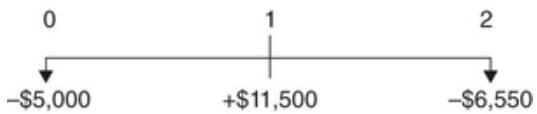
\includegraphics[max width=\textwidth]{2024_04_10_6f0546190ca30f08bc91g-2}
\end{center}

\section*{Cash Flows of Hypothetical Derivative Contract}
This cash flow pattern changes signs twice, once from negative to positive and once from positive to negative. There are two IRRs: $3.82 \%$ and $26.20 \%$. Both $3.82 \%$ and $26.20 \%$ satisfy the definition of the IRR because they set the present value of all cash inflows equal to the present value of all cash outflows. The net value of the present values of the cash inflows and outflows is illustrated in the next exhibit. Note that the line crosses the horizontal axis twice, defining two different IRRs.

With the two IRR solutions $3.82 \%$ and $26.20 \%$, there may be a temptation to think that the two IRRs can be somehow analyzed in unison to generate an intuitive feel for the derivative's attractiveness. But neither number is particularly useful, because the investment is really a combination of investing from period 0 to period 1 and borrowing from period 1 to period 2 . In this particular case, the cash flow patterns have a positive net value between the two IRRs, using discount rates between $3.82 \%$ and $26.20 \%$. But as a derivative, it is obvious that the cash flows to the other side of the derivative (the counterparty) would have the same numbers, but the signs of the cash flows would be reversed. In this case, the cash flows would be $+\$ 5,000,-\$ 11,500$, and $+\$ 6,550$. From the counterparty's perspective, the IRR solutions would still be exactly the same at $3.82 \%$ and $26.20 \%$. However, the deal's graph would appear as a mirror image, with negative net values between the two IRRs. As we would expect with a derivative deal, gains to one side of the contract would equal losses to the other side of the contract. Both sides would view the same IRRs because they used the same cash flows, but they would be looking at opposite cash flows and opposite net values. Therefore, using only the IRRs to decide if the derivative is beneficial is not possible.

\begin{center}
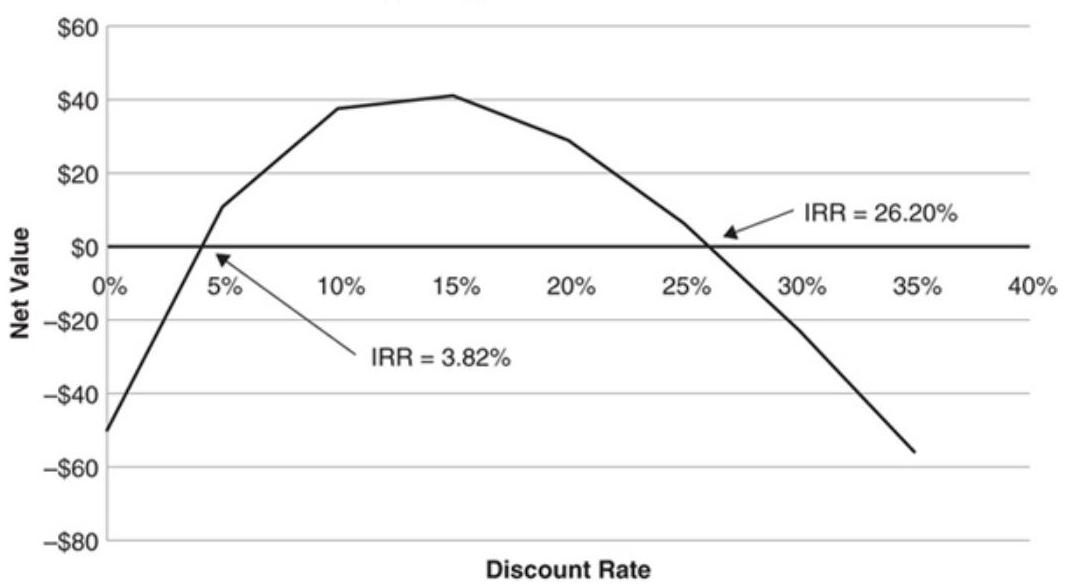
\includegraphics[max width=\textwidth]{2024_04_10_6f0546190ca30f08bc91g-3}
\end{center}

An Example of Multiple IRRs

\section*{Comparing Investments Based on IRRs}
The previous section reviewed the difficulties of computing and interpreting IRRs when an investment offers a complex cash flow stream. But even if the investments being analyzed offer simplified cash flow streams (a cash outflow followed only by cash inflows), the IRR method of measuring investment performance has serious challenges. This section details the major challenges of comparing investments based on IRR.

The major challenge with comparing IRRs across investments occurs when investments have scale differences. Scale differences are when investments have unequal sizes and/or timing of their cash flows. When comparing investments with different scales, an investment with a higher IRR may be inferior to an investment with a lower IRR.

The following is a simple example that illustrates the problems that occur when comparing IRRs. Assume that a bank is offering high initial yields on a limited-time basis to induce investors to open a new account. Investors are allowed to open only one account. The example includes three types of accounts, each with the following interest rates and restrictions on time and amount:

\begin{itemize}
  \item Account Type A: Receive $100 \%$ annualized interest for the first day on the first $\$ 10,000$.
  \item Account Type B: Receive $100 \%$ annualized interest for the first year on up to $\$ 10$.
  \item Account Type C: Receive $20 \%$ annualized interest for the first year on up to $\$ 10,000$.
\end{itemize}

The IRR of alternatives A and B is $100 \%$, whereas the IRR of alternative C is only $20 \%$. However, alternative A has very small scale due to a time limitation of one day (timing), and alternative B has very small scale due to a cash flow size limitation of $\$ 10$ (size). If annualized market interest rates are $5 \%$, alternative A has a net present value of less than $\$ 30$, and alternative B has an NPV of less than $\$ 10$. Alternative $C$ has an NPV of about $\$ 1,500$, even though its IRR is only one-fifth that of the other two alternatives. The reason for this is that although all three alternatives have favorable IRRs, alternative $\mathrm{C}$ has much larger scale.

In this example, it is better to receive a lower rate on a large scale. In actual investing, scale differentials can be complex and subtle. In judging when a larger scale is worth a sacrifice in return, approaches to investments using the NPV method offer substantial potential in evaluating investment opportunities of different scales. But in alternative investments, especially private equity, IRR is the standard methodology, and scale differentials represent a challenge in ranking performance.

\section*{IRRs Should Not Be Averaged}
Another challenge to using IRRs involves aggregation. Aggregation of IRRs refers to the relationship between the IRRs of individual investments and the IRR of the combined cash flows of the investments. Suppose that one investment earns an IRR of $15 \%$ and another earns an IRR of $20 \%$. What would the IRR be of a portfolio that contained both investments? In other words, if the cash flows of two investments are combined into a single cash flow pattern, how would the IRR of the combination relate to the IRRs of the individual investments? The answer is not immediately apparent, because the IRR of a portfolio of two investments is not generally equal to a value-weighted average of the IRRs of the constituent investments. If the cash flows from two investments are combined to form a portfolio, the IRR of the portfolio can vary substantially from the average of the IRRs of the two investments.

This section demonstrates the difficulty of aggregating IRRs, and the following extreme example illustrates the challenges vividly. Consider the following three investment alternatives:

\begin{center}
\begin{tabular}{|lccc|}
\hline
Name & $\mathrm{CF}_{0}$ & $\mathrm{CF}_{1}$ & IRR \\
\hline
Investment A & -100 & +110 & $10 \%$ \\
Investment B & +150 & -150 & $0 \%$ \\
Investment C & +50 & -50 & $0 \%$ \\
\hline
\end{tabular}
\end{center}

The IRRs of the three alternatives are easy to compute because each investment simply offers two cash flows: one at time period 0 and one at time period 1 . Using Equation 2 in the Internal Rate of Return lesson, the IRR for a one-period investment is found by solving the equation $0=C F_{0}+C F_{1} /(1+$ IRR $)$, which generates the equation

$$
\operatorname{IRR}=\left(C F_{1} /-C F_{0}\right)-1
$$

Inserting the values for Investment A $\left(C F_{0}=-100, C F_{1}=+110\right)$ generates the IRR of $10 \%$, shown in the IRR column. Investments $\mathrm{B}$ and $\mathrm{C}$ both have $C F_{0}=-C F_{1}$, so the IRRs of both Investment $B$ and Investment $C$ are $0 \%$. One might expect that combining Investment $A$ with either Investment $B$ or Investment $C$ would generate a portfolio with an IRR between $0 \%$ and $10 \%$ because one investment in the portfolio would have a stand-alone IRR of $10 \%$, as with Investment A, and the other would have a stand-alone IRR of 0\%, as in the case of either Investment B or C. But IRRs can generate unexpected results, as indicated by the following analysis:

\begin{center}
\begin{tabular}{|lllc|}
\hline
Name & CF $_{0}$ & CF $_{1}$ & IRR \\
\hline
Investment A + B & +50 & -40 & $-20 \%$ \\
Investment A + C & -50 & +60 & $+20 \%$ \\
\hline
\end{tabular}
\end{center}

The computations simply sum the cash flows of two investments and compute the single-period IRR of the aggregated cash flows. The IRR of combining Investments $A$ and $B$ is $-20 \%$, and the IRR of combining Investments $A$ and $C$ is $+20 \%$. The IRRs of both combinations are well outside the range of the IRRs of the individual investments in each portfolio. What generates the unexpected result in this example is that Investments B and $\mathrm{C}$ begin with cash inflows and end with cash outflows (i.e., they are borrowing investments). But in practice, alternative investments, such as commodity or real estate derivatives and private equity, can have cash flow patterns sufficiently erratic to cause serious problems with aggregation of IRRs.

\section*{IRR and the Reinvestment Rate Assumption}
Even if all the investments have simplified cash flow patterns without borrowing or multiple sign change problems, the IRR does not necessarily rank investments accurately. The use of the IRR to rank investment alternatives is often said to rely on the reinvestment rate assumption. The reinvestment rate assumption refers to the assumption of the rate at which any cash flows not invested in a particular investment or received during the investment's life can be reinvested during the investment's lifetime. If the assumed reinvestment rate is the same rate of return as the investment's IRR, then no ranking problem exists.

Suppose that Investment A offers an attractive IRR of $25 \%$ compared with the $20 \%$ IRR of Investment B. As previously discussed, it is possible that an investor would select Investment B over Investment A if Investment B offers a larger scale, meaning more money invested for longer periods of time. But if an investor who selects Investment A is able to invest additional funds at a $25 \%$ rate of return and is able to reinvest any cash flows from Investment A at the $25 \%$ rate, then the scale problem vanishes, and IRRs can be used to rank investments effectively. In practice, there would typically be no reason to assume that cash inflows could be reinvested at the same rate throughout the project's life, so ranking remains a problem. The reinvestment rate assumption is addressed by the modified IRR discussed in the next section.

\section*{Modified Internal Rate of Return}
The key method (other than net present value) to address the challenges of the IRR approach is the modified IRR approach. The modified IRR approach addresses the challenges of multiple IRRs and the restrictiveness of the reinvestment assumption in the IRR approach by discounting all project cash outflows into a present value using a financing rate, compounding all cash inflows into a future value using an assumed reinvestment rate, and calculating the modified IRR as the discount rate that sets the absolute values of that future value and that present value equal to each other. Consider a project such as one that might occur in a private equity investment that has cash flows that alternate in sign through time, as depicted in the next exhibit, Cash Flows for Private Equity Investment.

\begin{center}
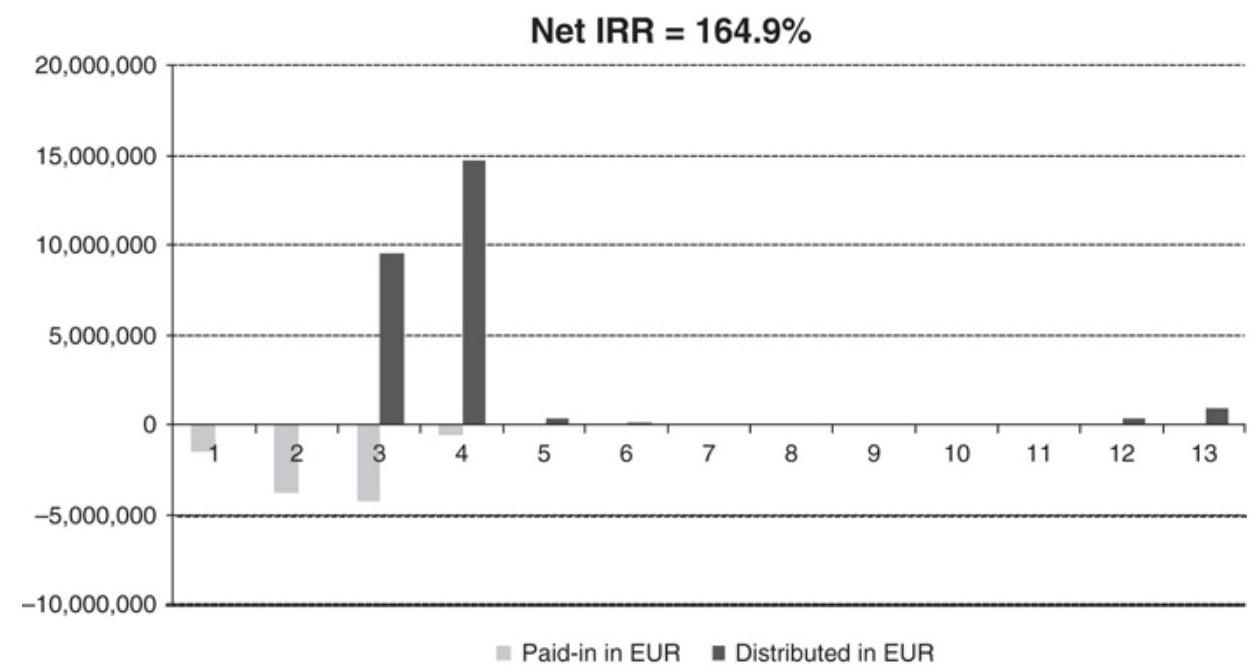
\includegraphics[max width=\textwidth]{2024_04_10_6f0546190ca30f08bc91g-4}
\end{center}

\section*{Cash Flows for Private Equity Investment}
Implicit in the use of IRR as a performance measure is the assumption that net distributions (such as those received in years 3 and 4 of the previous exhibit, Cash Flows for Private Equity Investment) can be reinvested at the IRR (164.9\%!). For a project like the one illustrated, the assumption would likely be very unrealistic and would be very misleading if IRR were used to rank dissimilar projects. To address this problem, the modified IRR (MIRR) imposes user-specified rates to compound all cash inflows forward to the project's termination date and discount all cash outflows back to the project's inception date. The next exhibit, Modified IRR Example illustrates the result: a single present value of the cash outflows at time 0 and a single future value of the cash inflows at time $T$.

\begin{center}
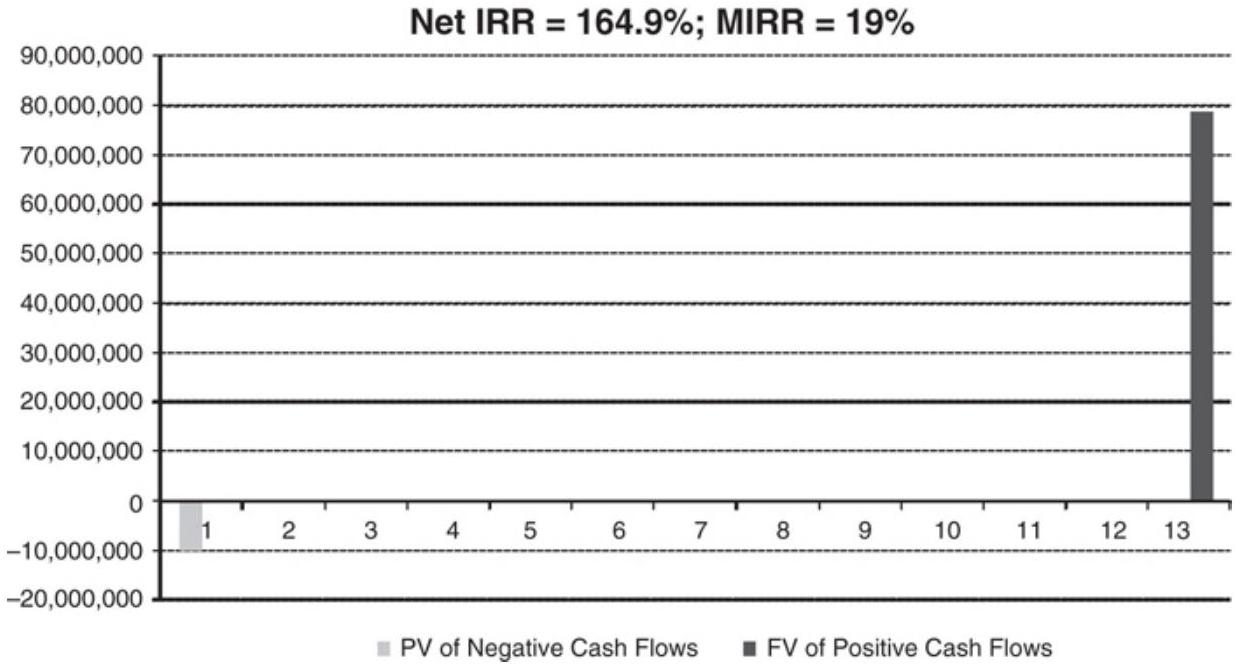
\includegraphics[max width=\textwidth]{2024_04_10_6f0546190ca30f08bc91g-5}
\end{center}

\section*{Modified IRR Example}
The modified IRR (19\%) is then very simply calculated as the discount rate that equates the future value of the cash flows to the present value of the negative cash flows (with both signs positive). Mathematically, the modified internal rate of return over the project's $T$ years, $M I R R_{T}$, is found by solving the following equation:


\begin{equation*}
\operatorname{MIR} R_{T}=\left(\frac{\text { FV of Positive Cash Flows Using the Reinvestment Rate }}{- \text { PV of Negative Cash Flows Using the Cost of Capital }}\right)^{\frac{1}{T}}-1 \tag{1}
\end{equation*}


where $T$ is the number of years between the project's first and last cash flows. Note that the negative sign in the denominator of the above Equation 1 is used to highlight the need to use absolute values in place of negative cash flows. Equation 2 expands the previous equation to provide needed details.


\begin{equation*}
\operatorname{MIRR}_{T}=\left(\frac{\sum_{t=0}^{T} D_{t} \times(1+R R)^{T-t}}{\left|\sum_{t=0}^{T} \frac{C_{t}}{(1+C C)^{t}}\right|}\right)^{\frac{1}{T}}-1 \tag{2}
\end{equation*}


where $D_{t}$ is the distribution in year $t, C_{t}$ is the contribution in year $t, R R$ is the expected reinvestment rate for the period until time $T, C C$ is the investors' cost of capital through period $T$, and MIRR ${ }_{T}$ is the modified IRR. Equation 2 can be solved for MIRR easily with most financial and nonfinancial calculators given the values of the contributions, distributions, $R R$, and $C C$.

The $R R$ is used to find the total value that the distributions would accrue to at the end of the project's life if they were all reinvested at $R R$. The $C C$ is used to find the aggregated initial cost of financing the project's contributions. To the extent that $R R$ and $C C$ are accurate and properly reflect implications of the various risks involved, the MIRR $_{T}$ can be viewed as an indication of the return earned from the excess of the accrued distributions over the project's financing costs.

\section*{Advantages and Disadvantages of Modified Internal Rate of Return}
There is considerable debate with regard to the meaning and selection of the rates $R R$ and $C C$ in Equation 2. $R R$ is usually interpreted as the firm's reinvestment rate -the expected return the firm could be expected to earn by reinvesting the distributions that it receives from the project. $C C$ is often interpreted as the firm's marginal cost of capital-the expected cost of financing the project's contributions. However, different commentators and practitioners differ in their approaches, including the possibility that either or both of the rates are set equal to market rates.

The two major advantages to the MIRR approach are that it addresses two important deficiencies with IRR.

First, as illustrated in the last exhibit, Modified IRR Example, by imposing $R R$ and $C C$ for discounting the cash outflows and compounding the cash inflows, the computation of the metric (i.e., the MIRR) becomes a simple rate of return computation with no possibility of multiple solutions. Thus, the MIRR approach overcomes the multiple IRR issue that can exist when a project's cash flows have multiple sign changes through time.

Second, the MIRR approach overrides the implicit reinvestment assumption of the traditional IRR model (that cash distributions from a project can be reinvested at a rate equal to the project's IRR). When various projects are ranked by IRR, the reinvestment assumption implicit in IRR can cause the rankings to differ from those generated by the net present value rule (which is generally found to be superior). The MIRR approach addresses this problem by imposing a user-specified reinvestment rate, $R R$. In the case of private equity it makes sense that the return that is earned from reinvesting the distributions into a new project can be quite different from the return earned on the extant project.

However, the MIRR approach is viewed as having substantial disadvantages that make it a rarely used approach relative to the IRR. Note that the values of $C C$ and $R R$ chosen by the user drive the value of the resulting MIRR. For example, a high $R R$ combined with a high $C C$ will cause the MIRR to be high by increasing the future value of the distributions and lowering the present value of the contributions. So unlike IRR, MIRR is driven by user-selected rates ( $R R$ and $C C$ ) that conceptually are unrelated to the project.

As an example of the difficulties with the MIRR approach, consider what happens when a $\$ 1$ distribution in Year 10 is added to the cash flows in Application A. Common sense indicates that adding a single dollar to the cash inflows in year 10 should cause performance metrics to rise very slightly. In fact, the IRR rises from $14.38 \%$ to $14.42 \%$, indicating the nearly trivial but beneficial nature of receiving a distant dollar. But the MIRR falls substantially from $12.83 \%$ to $11.42 \%-a$ huge decline and in the intuitively wrong direction. The extra five years added to the project's lifetime drives the MIRR closer to the $R R$. In fact, as the location of the extra dollar is moved into the future (i.e., the project's lifetime is expanded with a trivial cash flow), the MIRR approaches the $R R$ because the addition of a distribution even of only $\$ 1$ causes the approach to compound all of the other distributions to the project's termination. In Application A the assumed $R R$ of $10 \%$ is less than the original project's IRR and MIRR. Therefore, stretching the project's lifetime by adding a distant dollar lowers the MIRR toward the RR even though the addition of an extra dollar of cash should cause a performance measure to increase.

In summary, the MIRR approach solves the problem of the IRR approach of multiple solutions and in some cases can help alleviate distortions caused by the reinvestment rate assumption. However, the results of the MIRR approach can be very sensitive to the reinvestment rate (RR) and financing cost (CC) assumed, and can generate perverse rankings relative to NPV approach.

\section*{Time-Weighted Returns versus Dollar-Weighted Returns}
The purpose of this section is to provide details regarding time-weighted returns versus dollar-weighted returns. Briefly, time-weighted returns are averaged returns that assume that no cash was contributed or withdrawn during the averaging period, meaning after the initial investment. Dollar-weighted returns are averaged returns that are adjusted for and therefore reflect when cash has been contributed or withdrawn during the averaging period. The IRR is the primary method of computing a dollar-weighted return.

When evaluating the return of hedge funds, mutual funds, or any investment, it's important to recognize the distinction between the time-weighted return, which is similar to what is reported on performance charts in marketing literature and client letters, and the dollar-weighted return, which represents what the average investor actually earned; the two can be very different.

Suppose there is a hedge fund that in year 1 starts with $\$ 100$ million of AUM (assets under management). Let's further suppose that the hedge fund generates an average annual return of $20 \%$ for each of its first three years. With such a performance history, the hedge fund attracts quite a bit of new capital. Let's assume that the hedge fund attracts $\$ 200$ million in new assets for year 4, another $\$ 200$ million for year 5 , and nothing in year 6 . Unfortunately, the new capital does not help the hedge fund manager maintain the fund's stellar performance, and the manager earns $0 \%$ in years 4,5 , and 6 . If we use time-weighted returns over this six-year period, the hedge fund manager has an average annual return of $9.5 \%$ :

$$
(1.2 \times 1.2 \times 1.2 \times 1.0 \times 1.0 \times 1.0)^{\frac{1}{6}}-1=1.095-1=9.5 \%
$$

In effect, the time-weighted return assumes that a single investment (e.g., \$1) was made at the beginning of the period and was allowed to grow with positive returns and decline with negative returns until the end of the measurement period, with no cash withdrawals or additional contributions. The rate that equates the initial value with the accumulated value is the time-weighted average return, and it is somewhat near the arithmetic average annual return (in this case, $10 \%$ per year). The idea is that a single sum of money invested at the start of the first year and allowed to remain in the fund until the end of the last year would accumulate to the same value as if it had been invested at a fixed return of $9.5 \%$ per year, ignoring rounding.

But in practice, investors often contribute additional cash (i.e., make additional investments) or withdraw cash (e.g., liquidate part of the investment or receive cash distributions) during the time period under analysis. Their average returns depend on whether the amount of money invested was highest during the highperforming periods or during the low-performing periods. Dollar-weighted returns adjust the average annual performance for the amount of cash invested each year. In the case of the hedge fund, an investor who had much more cash in the fund in the early years than in the later years would earn more than an investor whose money was primarily invested in the last three years, when the fund generated $0 \%$ returns.

Dollar-weighted returns can be computed for each investor using investors' cash flows into and out of the hedge fund. The total cash flows into and out of the fund for all investors can be used as an indication of the performance of an average investor. The dollar-weighted return that individual investors experience depends on their cash contributions and withdrawals.

When the timing of the aggregated cash flows for the entire hedge fund is taken into account, the bulk of the hedge fund's assets earned a $0 \%$ return in years 4,5 , and 6. The example shows that only the first $\$ 100$ million earned the great rates of return of the first three years. The $\$ 400$ million that flowed into the hedge fund in years 4 and 5 earned a $0 \%$ return. When the timing of the aggregated cash flows is taken into account, the dollar-weighted return (solving for the IRR with cash flows reinvested) is only $4.3 \%$. The IRR is found in this case with $C F_{0}=-100, C F_{1}=0, C F_{2}=0, C F_{3}=-200, C F_{4}=-200, C F_{5}=0$, and $C F_{6}=+572.8$; that is, $C F_{6}$ is found as: $[(100 \times$ $1.2 \times 1.2 \times 1.2)+200+200]$.

Investment managers are best evaluated on time-weighted returns, as these managers should not be held accountable for the cash flow decisions of their investors. Investors should evaluate their own investment results using dollar-weighted returns based on the cash flows from their particular investment pattern.


\end{document}